\documentclass[11pt]{article}
\usepackage[margin=1in]{geometry}
\usepackage{graphicx}
\usepackage{float}
\usepackage{booktabs}
\usepackage{listings}
\usepackage{xcolor}
\usepackage{caption}
\usepackage{hyperref}

\definecolor{codegray}{gray}{0.95}
\lstset{
  backgroundcolor=\color{codegray},
  basicstyle=\ttfamily\small,
  frame=single,
  breaklines=true,
  showstringspaces=false,
  postbreak=\mbox{\textcolor{red}{$\hookrightarrow$}\space}
}

\title{Operating Systems Lab Assignment: Thread-Safe Data Structures}
\author{Cameron Cleveland}
\date{October 21, 2025}

\begin{document}
\maketitle

\section{Introduction}
This report documents the implementations and analyses for the thread-safe data structures lab assignment, covering thread-safe queue and stack implementations, Producer-Consumer and Undo-Redo use cases, and additional exercises.

\section{Exercise 1: Thread-Safe Queue and Stack}
\lstinputlisting[language=C++]{thread_safe_data_structures.cpp}
\textbf{Explanation}: The queue and stack were made thread-safe by using a single mutex to lock each operation. Every function (push, pop, size, empty) is wrapped with a \texttt{std::lock\_guard<std::mutex>} to ensure that only one thread can access or modify the structure at a time. In the Producer-Consumer simulation, multiple producers push messages while consumers continuously pop them until all messages are processed. The Undo-Redo system uses two stacks: edits push the previous state onto the undo stack and clear the redo stack, while undo and redo operations swap states safely between the two.

\textbf{Analysis}: This design ensures correctness and simplicity but limits concurrency because each operation holds the same lock. The termination logic checks both production count and emptiness, which works but could race under heavier loads. Using condition variables for blocking consumers would prevent busy-waiting and improve efficiency. Overall, the exercise highlights the balance between safety and performance in synchronization.

\textbf{Screenshot}: Include a screenshot of compiling and running thread\_safe\_data\_structures.cpp.
\begin{figure}[h]
    \centering
    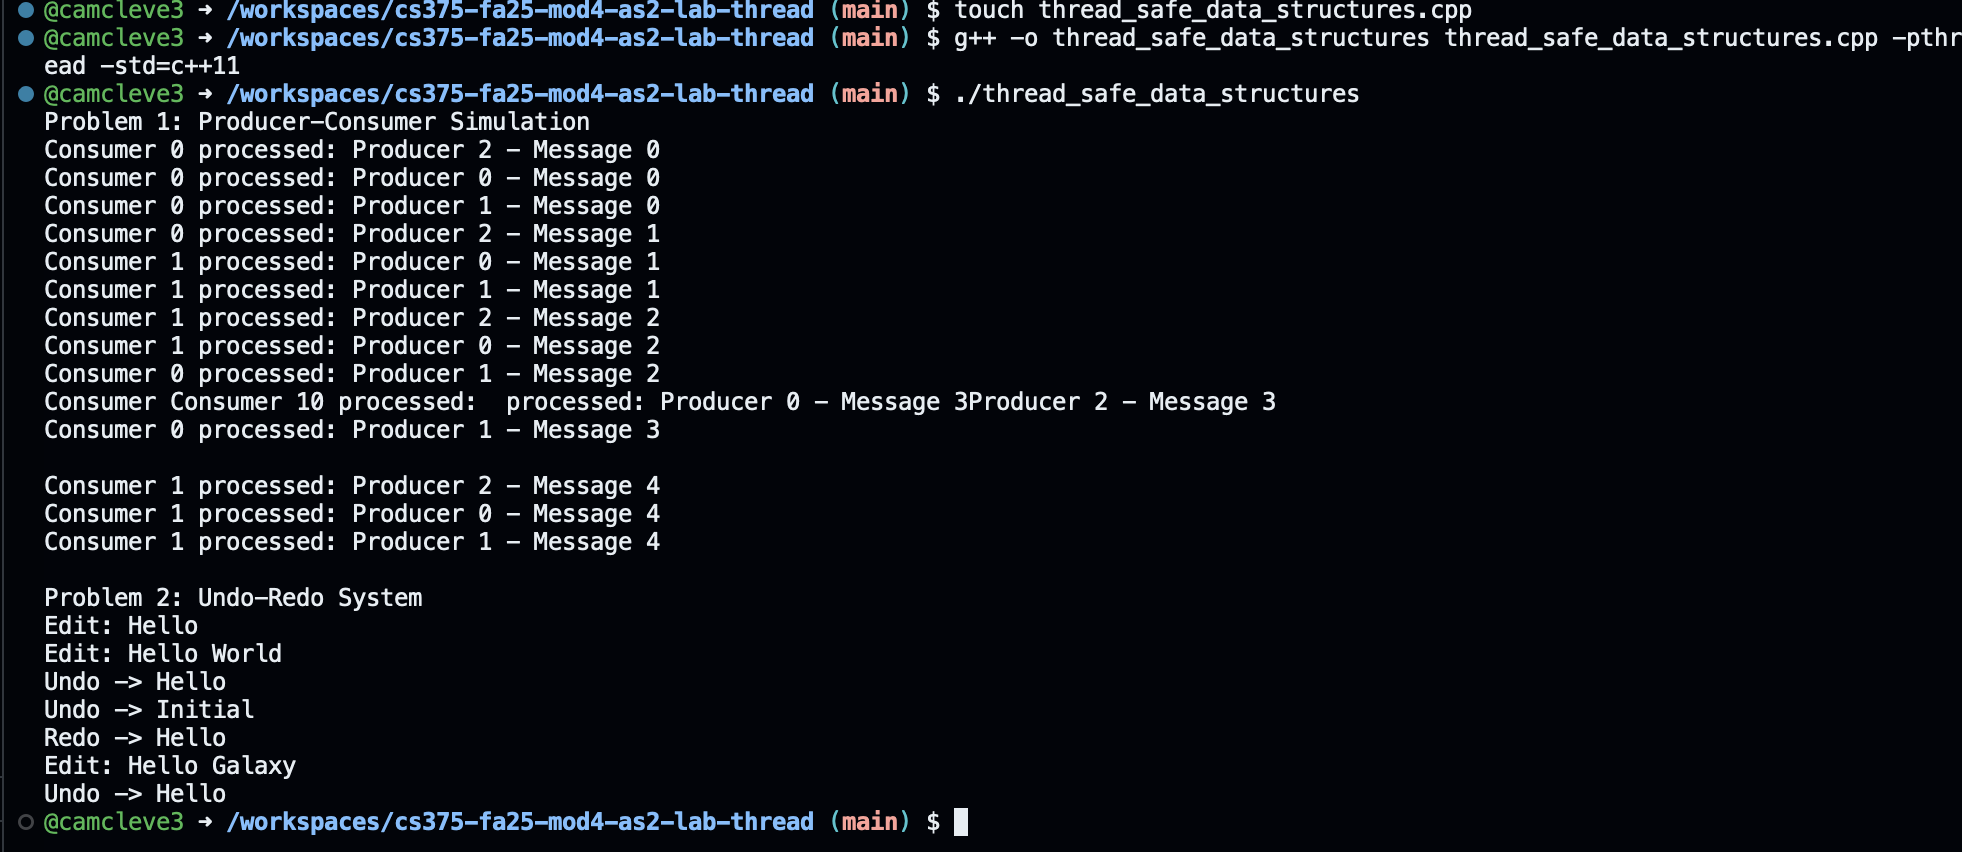
\includegraphics[width=\textwidth]{pic1.png}
    \caption{Compilation and execution of thread\_safe\_data\_structures.cpp}
\end{figure}

\section{Exercise 3: Thread-Safe Priority Queue}
\lstinputlisting[language=C++]{priority_queue.cpp}
\textbf{Explanation}: The priority queue uses a \texttt{std::priority\_queue} container wrapped with a mutex to protect insertion and removal. Each operation locks the queue before accessing the heap, maintaining order and preventing race conditions even when multiple threads push or pop simultaneously.

\textbf{Analysis}: The implementation is safe and correct but fully serialized, every push and pop operation competes for the same lock. For improved concurrency, condition variables could be used to block consumers until data becomes available. A more scalable solution might involve multiple internal queues or a lock-free heap, though this adds complexity beyond the lab scope.

\textbf{Screenshot}: Include a screenshot of compiling and running priority\_queue.cpp.
\begin{figure}[h]
    \centering
    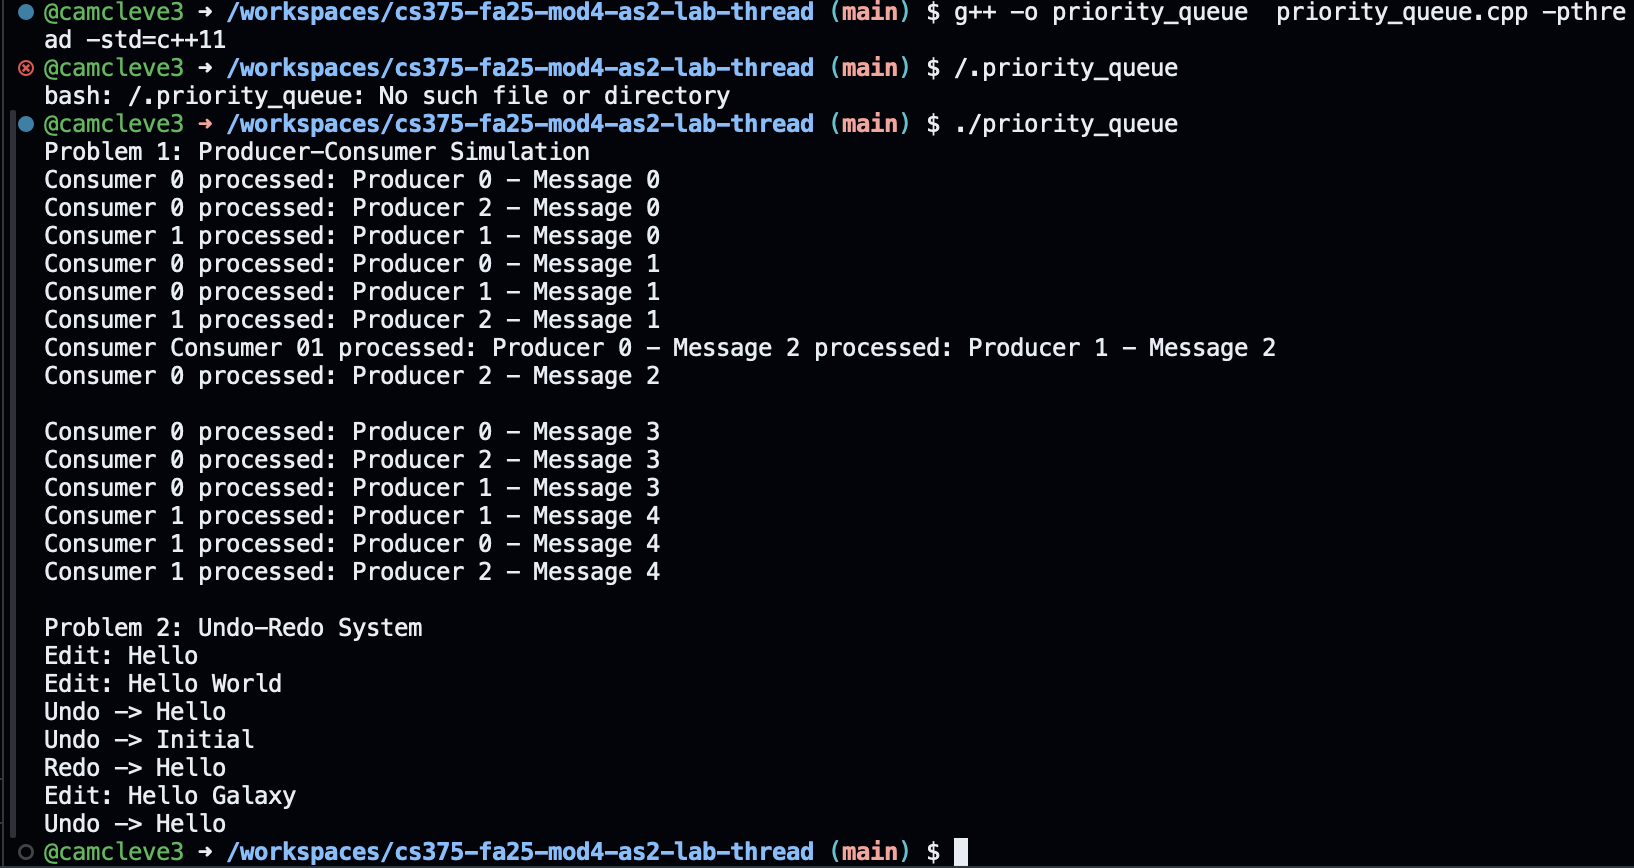
\includegraphics[width=\textwidth]{pic2.png}
    \caption{Compilation and execution of priority\_queue.cpp}
\end{figure}

\section{Exercise 4: Thread-Safe Circular Buffer}
\lstinputlisting[language=C++]{circular_buffer.cpp}
\textbf{Explanation}: The circular buffer implementation uses a fixed-size vector with head, tail, and count indices. One mutex controls access, while two condition variables , \texttt{not\_full} and \texttt{not\_empty} , handle producer and consumer synchronization. Producers wait when the buffer is full, and consumers wait when it’s empty, ensuring no overwriting or reading invalid data.

\textbf{Analysis}: The buffer introduces natural backpressure, keeping memory usage predictable and enforcing balance between production and consumption. The main challenges were avoiding off-by-one index errors and ensuring condition variables were properly signaled. Updating shared state within a locked region and notifying afterward kept the behavior consistent. This implementation shows how condition variables enable efficient coordination without wasting CPU cycles.

\textbf{Screenshot}: Include a screenshot of compiling and running circular\_buffer.cpp.
\begin{figure}[h]
    \centering
    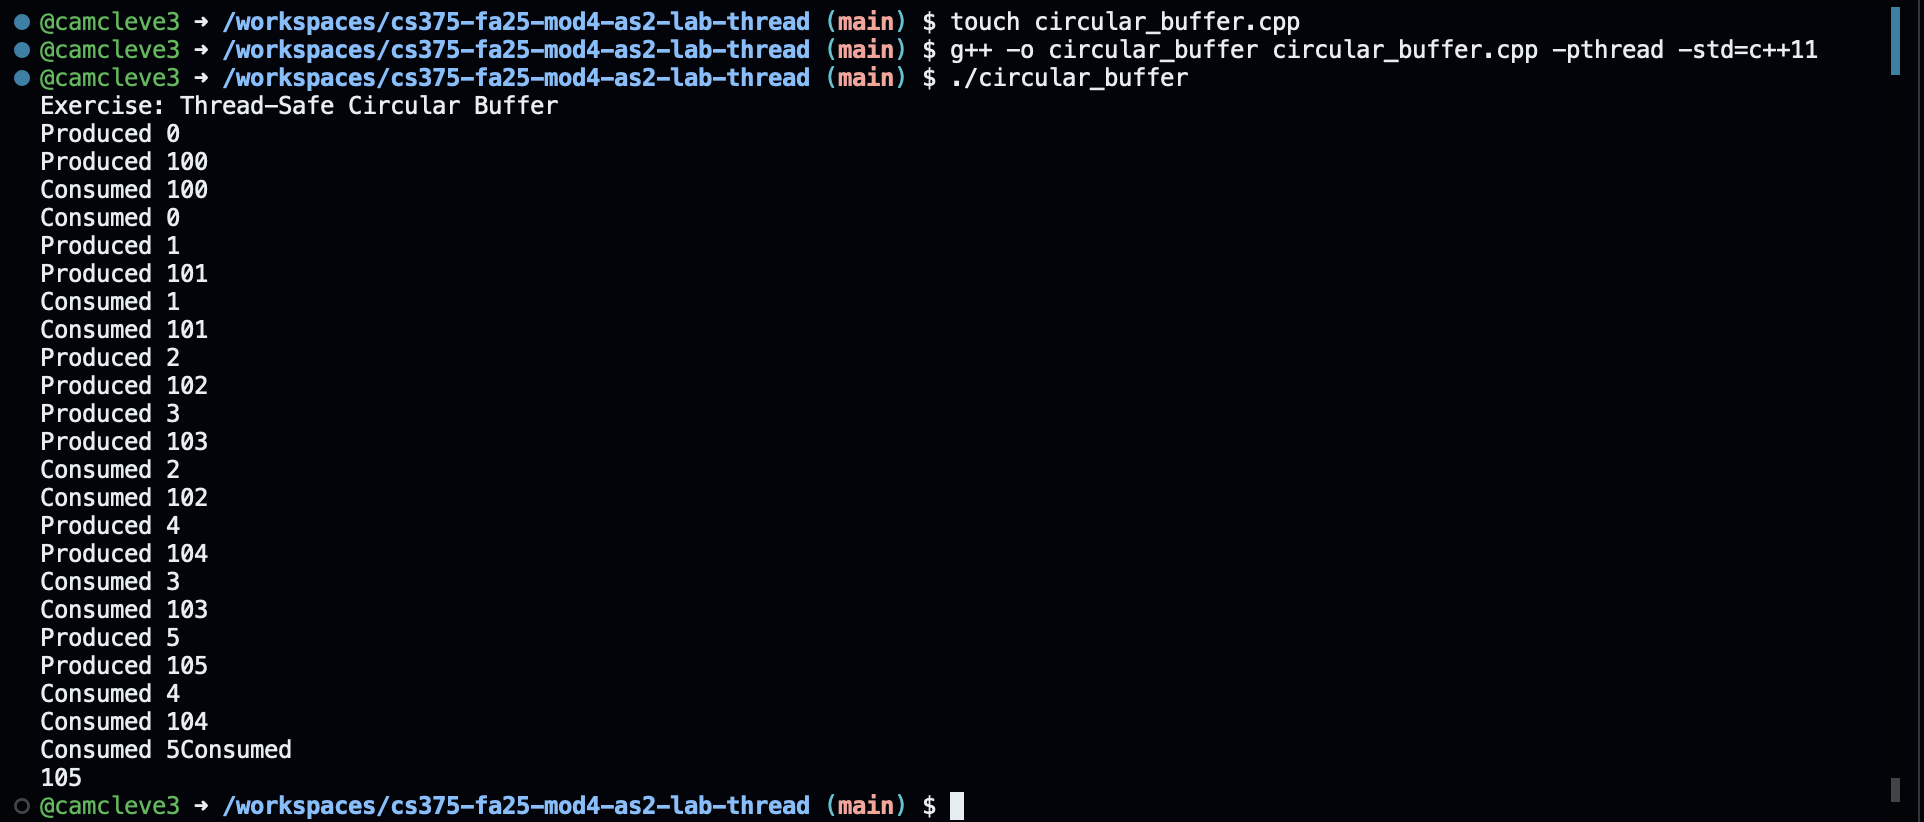
\includegraphics[width=\textwidth]{pic3.png}
    \caption{Compilation and execution of circular\_buffer.cpp}
\end{figure}

\section{Exercise 5: Thread-Safe Deque}
\lstinputlisting[language=C++]{thread_safe_deque.cpp}
\textbf{Explanation}: The deque supports operations from both ends and is synchronized with a single mutex that guards all operations. Each push and pop action locks the deque to maintain data consistency and prevent race conditions during concurrent access.

\textbf{Analysis}: While simple and correct, this design can become a bottleneck when multiple threads push and pop from both ends simultaneously. A refined version could use separate locks for the head and tail to reduce contention but would need strict ordering to avoid deadlocks. This exercise demonstrates the trade-offs between fine-grained locking complexity and overall thread safety.

\textbf{Screenshot}: Include a screenshot of compiling and running thread\_safe\_deque.cpp.
\begin{figure}[h]
    \centering
    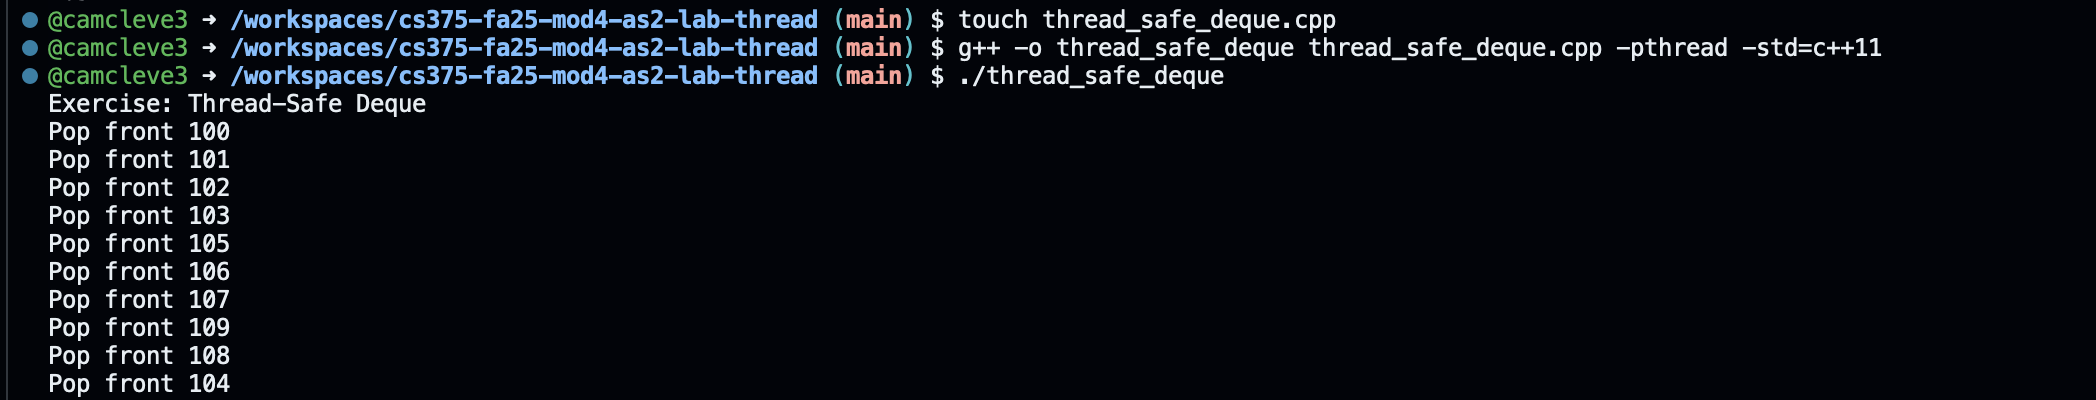
\includegraphics[width=\textwidth]{pic4.png}
    \caption{Compilation and execution of thread\_safe\_deque.cpp}
\end{figure}

\section{Exercise 6: Thread-Safe Linked List}
\lstinputlisting[language=C++]{thread_safe_linked_list.cpp}
\textbf{Explanation}: The linked list is implemented with coarse-grained locking, using one mutex to guard the entire structure. Each operation (\texttt{push\_front}, \texttt{pop\_front}, \texttt{size}, and \texttt{empty}) locks the list, ensuring safe pointer updates and consistent traversal during concurrent modifications.

\textbf{Analysis}: This design is reliable and easy to understand, making it ideal for demonstrating basic synchronization concepts. However, scalability is limited since only one thread can modify or read at a time. In real-world systems, fine-grained or lock-free approaches would improve performance but require complex memory management to handle concurrency safely. For the purposes of this lab, the coarse lock approach provides a clear foundation for thread-safe list operations.

\textbf{Screenshot}: Include a screenshot of compiling and running thread\_safe\_linked\_list.cpp.
\begin{figure}[h]
    \centering
    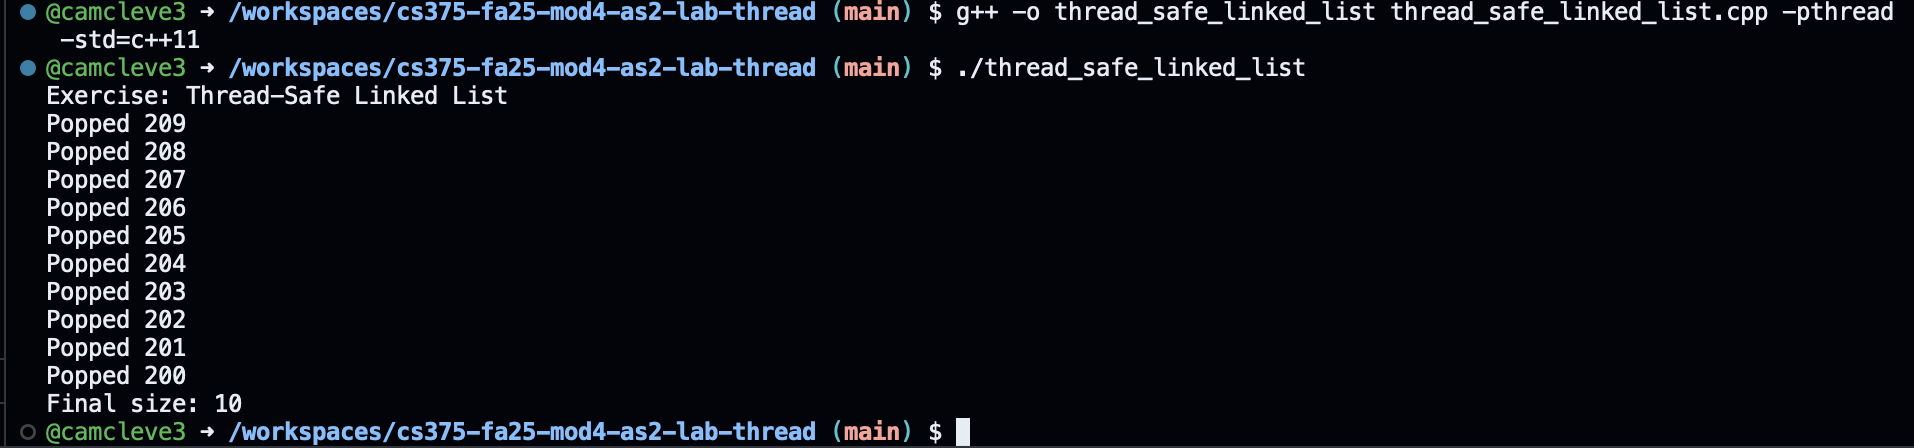
\includegraphics[width=\textwidth]{pic5.png}
    \caption{Compilation and execution of thread\_safe\_linked\_list.cpp}
\end{figure}

\end{document}